\newcommand{\medianWCStartAlexa}{876}
\newcommand{\medianWCEnd}{1522}
\newcommand{\medianFKStart}{11.9}
\newcommand{\medianFKEnd}{13.2}

\section{Document-level trends}
\label{sec:doclevstatstime}

We examine how length, readability, and updates have changed over time. Because 
most of the privacy policies in our corpus are
from 2009-2019, we focus most of our analysis on that time range.

\subsection{Comprehension}
\begin{figure}[t]
\centering
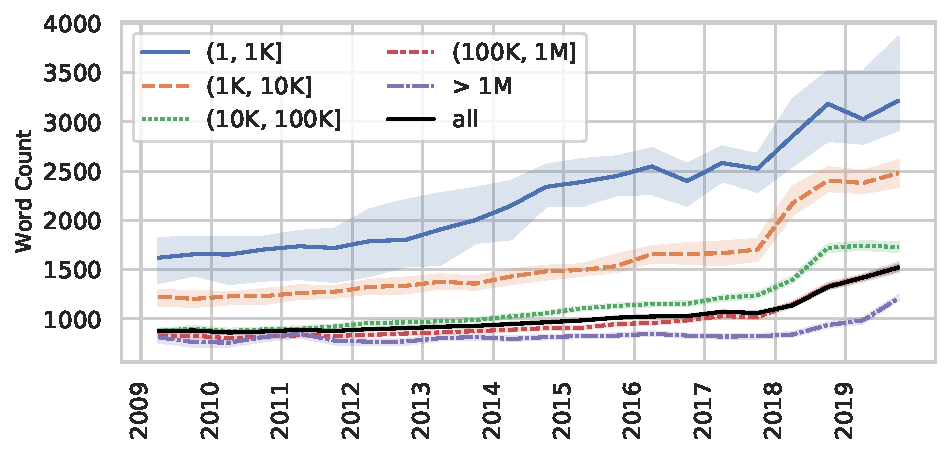
\includegraphics[width=0.99\columnwidth]{chapters/privacypolicies/figures/word-count-by-rank.pdf}
\caption{The median word count of policies binned by Alexa rank. The highlighted region in this and the following figures shows the 95\% confidence interval. Ranks are at the time of the snapshot.}
%\Description[Line plot of year vs word count]{The trend is generally slightly upwards and a similar shape across bins. Bins closer to 1 have more words.}
\label{fig:wordcount}
\end{figure}



{\bf Policy length.} Figure~\ref{fig:wordcount} shows the change in policy length as measured by word count. The median word count has increased gradually over time --- doubling between 2009A (\medianWCStartAlexa) and 2019B (\medianWCEnd) --- and more sharply in recent years, after the introduction of the GDPR. This trend holds for both popular and less popular websites. But the median hides a substantial variance: the 5\textsuperscript{th} percentile for word length is 248 words and the 95\textsuperscript{th} percentile is 3404 words. 
Our measurements for the top 10K are roughly consistent with the March 2016 measurements study by Degaling et al., but less so for their post-GDPR March 2018 measurements. Degaling et al. found the median privacy policy word count of the top 500 websites for 28 EU countries to be 2,145 in 2016 (our data: 1K: 2,691, 10K: 2,122) and 3,044 in 2018 (our data: 1K: 3,303, 10K: 2651) ~\cite{degeling2018we}. We believe the inconsistency is due to the difference in website sampling methods.




{\bf Readability.}
\label{sec:readability}
Several studies have shown that privacy policies are difficult to read~\cite{mcdonald2008cost,fabian2017large,milne2006longitudinal,li2012online}. 
Here we examine how readability has changed over time.
\begin{figure}
\centering
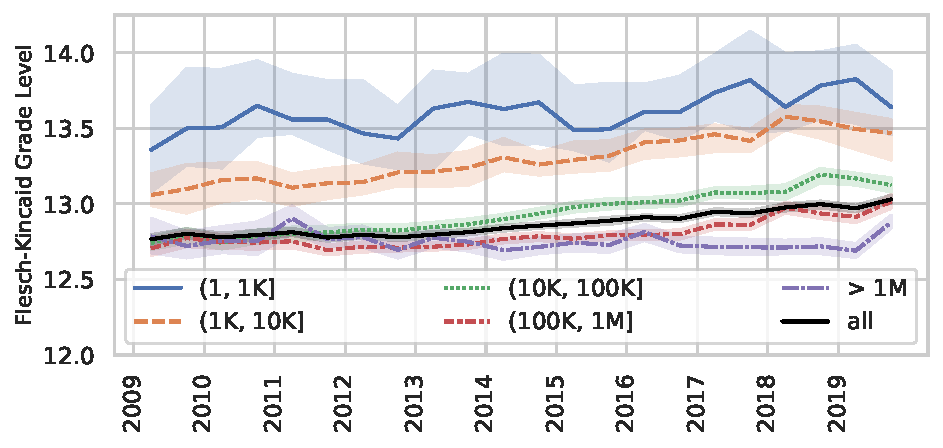
\includegraphics[width=1\columnwidth]{chapters/privacypolicies/figures/flesch_kincaid_dist.pdf}
\caption{Median Flesch-Kincaid grade level from 2009 to 2019, binned by Alexa rank. 
}
%\Description[Line plot of year vs Flesch Kincaid Grade level]{The trend is generally flat. Bins closer to 1 have a higher reading level.}
\label{fig:readability}
\end{figure}
We measured readability with the Flesch-Kincaid grade level (FKGL)~\cite{kincaid1975derivation}
using the \textit{py-readability-metrics} Python library~\cite{pyreadabilitymetrics}.
Our preprocessing involved removing non-sentence text such as headers, tables, and lists by writing a custom Markdown renderer using the \emph{Mistune}~\cite{mistune} Python library.

The FKGL measurements are shown in Figure~\ref{fig:readability}. The median readability score has risen more than a grade level from 2000A (\medianFKStart) to 2019B (\medianFKEnd). More popular websites have less readable policies.

In comparison, Li et al.~\cite{li2012online} measured the reading difficulty of privacy policies for websites for the 30 Dow Jones companies in 2012, finding an average FKGL of 13.33, which is similar to our findings for top 1K and top 10K websites.





\subsection{Privacy policy updates}
We measured the percentage of privacy policies updated in each interval.
To determine if these changes align with shifts in the language of privacy policies, we also measured terms that have experienced changes in their usage at each interval.

\textbf{Privacy policy updates.}
\label{sec:policy-updates}
\begin{figure}[]
\centering
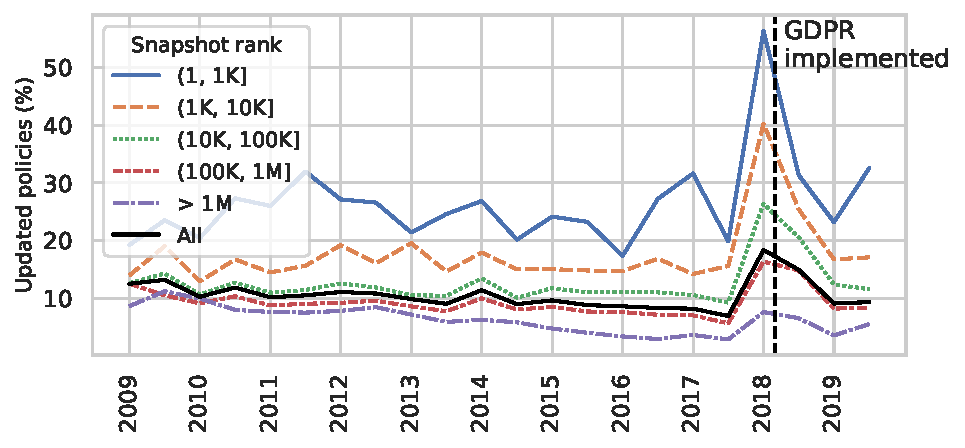
\includegraphics[width=0.99\columnwidth]{chapters/privacypolicies/figures/policy-updates.pdf}
\caption[Caption]{Percentage of privacy policies updated per interval.\protect\footnotemark}

%\Description[Line plot of year vs percentage of policies updated]{While jagged, the trends are relatively stable. Bins closer to 1 have more updated policies. There is a large spike shortly before GDPR is implemented.}

\label{fig:pct-policy-update}
\end{figure}
\footnotetext{We excluded snapshots for which we have a gap in the previous interval from Figure~\ref{fig:pct-policy-update}, since determining the exact time of the updates was not possible.}
Figure~\ref{fig:pct-policy-update} shows the percentage of updated policies, considering
only the~\emph{significant} updates, where the fuzzy similarity ratio~\cite{fuzzywuzzy} of consecutive policy snapshots is less than or equal to 95\%
~\cite{linden2020privacy}.
The spike in 2018 indicates the GDPR's substantial impact on privacy policies.  Although the figure shows that
popular websites update their policies more frequently,
the GDPR appears to have caused a major uptick across all rank buckets. 

\textbf{Change-point concentration.} 
To 
investigate the changes in privacy policy language and vocabulary,
we counted the number of n-gram frequency change-points detected by the PELT algorithm~\cite{killick2012optimal}, using the \textit{ruptures} library~\cite{ruptures}. Change point detection algorithms originate from the signal processing literature, and are designed to identify when a time-series signal has experienced a failure~\cite{picard1985testing}. In our case, n-gram frequency is the signal, and the ``failures'' are events that cause a shift in the usage.


We counted the number of change-points at each interval for lemmatized 1-grams and 8-grams with a document frequency of at least $0.01$ in at least one interval.
Figure~\ref{fig:changepoints} shows that the change points for n-grams concentrate around GDPR's introduction, following a similar trend to document level updates in Figure~\ref{fig:pct-policy-update}. This indicates that not only are websites updating their policies, but that the vocabulary used in privacy policies was forced to evolve due to the GDPR.


\textbf{Validation.} To verify that the increase in privacy policy updates we observed in 2018A was related to the GDPR, we took a list of GDPR-related phrases identified by Degeling et al.~\cite{degeling2018we}, plus the phrases “GDPR” and “General Data Protection Regulation,” and selected the subset of 20 phrases with a relative document frequency of less than 1\% in 2015A. We found that documents in 2018A containing at least one of these 20 GDPR-related phrases had a mean update length of 136 new lines, compared to 15 new lines in documents without these phrases, where “update length” is the number of added lines minus the number of deleted lines. The quartile boundaries were at, respectively, 0, 20, 129 and 0, 0, 0. This indicates that policies that contain GDPR-related terms were more likely to have a longer update in comparison to the prior version of the policy, supporting the link between the introduction of the GDPR and the increase in updates in 2018A.

\begin{figure}
    \centering
    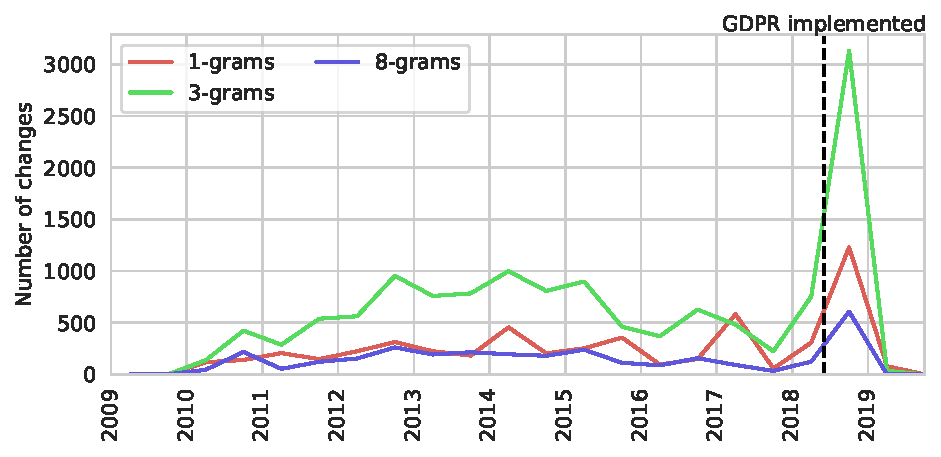
\includegraphics[width=.9\textwidth]{chapters/privacypolicies/figures/changepoints.pdf}
    \caption{Change point concentration. The y value is the number of frequent n-grams with change points in that interval for 1-grams, 3-grams, and 8-grams.}
    
%    \Description[Line plot of year vs number of changes]{There is a roughly arc shaped trend, with 3-grams being the most pronounced. There is a sharp spike right before GDPR is implemented.}
    \label{fig:changepoints}
\end{figure}
